	%-=-=-=-=-=-=-=-=-=-=-=-=-=-=-=-=-=-=-=-=-=-=-=-=
%
%        LOADING DOCUMENT
%
%-=-=-=-=-=-=-=-=-=-=-=-=-=-=-=-=-=-=-=-=-=-=-=-=

\documentclass[newPxFont,pagenumber]{beamer}
\usetheme{sthlm}
%\usecolortheme{sthlmv42}

%-=-=-=-=-=-=-=-=-=-=-=-=-=-=-=-=-=-=-=-=-=-=-=-=
%        LOADING PACKAGES
%-=-=-=-=-=-=-=-=-=-=-=-=-=-=-=-=-=-=-=-=-=-=-=-=
\usepackage[utf8]{inputenc}
\usepackage[frenchb]{babel}
\usepackage[normalem]{ulem}
\usepackage{caption}
\captionsetup{font=scriptsize}
%\usepackage[font=footnotesize]{subcaption}
% in preamble
\usepackage{chronology}
\usepackage{pgf}
\usepackage{tikz}
\usetikzlibrary{arrows,automata}
\usepackage{array,multirow}
\usepackage{nameref}
\makeatletter
\newcommand*{\currentname}{\@currentlabelname}
\makeatother

\graphicspath{ {fig/} }

\usepackage[linesnumbered,ruled,vlined]{algorithm2e}
% add page number
%\usepackage[defaultsans]{cantarell}

\newcommand{\p}{\mathbb{P}}

\setbeamerfont{title}{series=\upshape}
\setbeamertemplate{footline}{\hfill\footnotesize\insertframenumber\hskip3pt\null\vskip3pt}

\newcommand{\argmax}{\mathop{\mathrm{argmax}}\limits}
\renewcommand{\max}{\mathop{\mathrm{max}}\limits}

\renewcommand{\event}[3][e]{%
  \pgfmathsetlength\xstop{(#2-\theyearstart)*\unit}%
  \ifx #1e%
    \draw[fill=black,draw=none,opacity=0.5]%
      (\xstop, 0) circle (.2\unit)%
      node[opacity=1,rotate=45,right=.2\unit] {#3};%
  \else%
    \pgfmathsetlength\xstart{(#1-\theyearstart)*\unit}%
    \draw[fill=black,draw=none,opacity=0.5,rounded corners=.1\unit]%
      (\xstart,-.1\unit) rectangle%
      node[opacity=1,rotate=45,right=.2\unit] {#3} (\xstop,.1\unit);%
  \fi}%

\addto\captionsfrench{%
\renewcommand{\figurename}{\scriptsize {\scshape Figure}}
\renewcommand{\tablename}{\scriptsize {\scshape Table}}
}

%-=-=-=-=-=-=-=-=-=-=-=-=-=-=-=-=-=-=-=-=-=-=-=-=
%        BEAMER OPTIONS
%-=-=-=-=-=-=-=-=-=-=-=-=-=-=-=-=-=-=-=-=-=-=-=-=

%\setbeameroption{show notes}

%-=-=-=-=-=-=-=-=-=-=-=-=-=-=-=-=-=-=-=-=-=-=-=-=
%
%	PRESENTATION INFORMATION
%
%-=-=-=-=-=-=-=-=-=-=-=-=-=-=-=-=-=-=-=-=-=-=-=-=

\title{\normalsize Extraction d'information à partir de décisions judiciaires}
\subtitle{\small Journées des Doctorants du LGI2P 22 juin 2017}
%\date{\small{\jobname}}
%\date{\today}
\date{Début de thèse: 15 Décembre 2015}
\author{\textbf{TAGNY NGOMPE Gildas\textsuperscript{\ref{lgi2p},\ref{chrome}}}, Sébastien Harispe\textsuperscript{\ref{lgi2p}}, Jacky Montmain\textsuperscript{\ref{lgi2p}}, Stéphane Mussard\textsuperscript{\ref{chrome}}, Guillaume Zambrano\textsuperscript{\ref{chrome}}}
%\institute{\small\textbf{Directeur}: Stéphane Mussard, Pr. (CHROME, Univ. Nîmes)  \\ \textbf{Co-directeur}: Jacky Montmain, Pr. (LGI2P, Ecole des Mines d'alès) \\ \textbf{Encadrants}: Guillaume Zambrano, Sébastien Harispe}
\institute{%\scriptsize  
\begin{enumerate}
\item LGI2P (École des mines d'Alès) \label{lgi2p}
\item CHROME EA 7352 (Université de Nîmes) \label{chrome}
\end{enumerate}
}

\hypersetup{
pdfauthor = {\author{}: tagnyngompe@gmail.com},
pdfsubject = {},
pdfkeywords = {},
pdfmoddate= {D:\pdfdate},
pdfcreator = {}
}

\begin{document}
\nocite{}
%-=-=-=-=-=-=-=-=-=-=-=-=-=-=-=-=-=-=-=-=-=-=-=-=
%
%	TITLE PAGE
%
%-=-=-=-=-=-=-=-=-=-=-=-=-=-=-=-=-=-=-=-=-=-=-=-=
\begin{frame}[plain]
	\titlepage
\end{frame}
%}
%-=-=-=-=-=-=-=-=-=-=-=-=-=-=-=-=-=-=-=-=-=-=-=-=
%
%	TABLE OF CONTENTS: Plan
%
%-=-=-=-=-=-=-=-=-=-=-=-=-=-=-=-=-=-=-=-=-=-=-=-=
\section*{Plan}
\begin{frame}[c]{\currentname}
\tableofcontents[hideallsubsections]
\end{frame}

\section{Motivations et objectifs}

\begin{frame}[c]{Les juristes analysent les décisions afin d'anticiper}
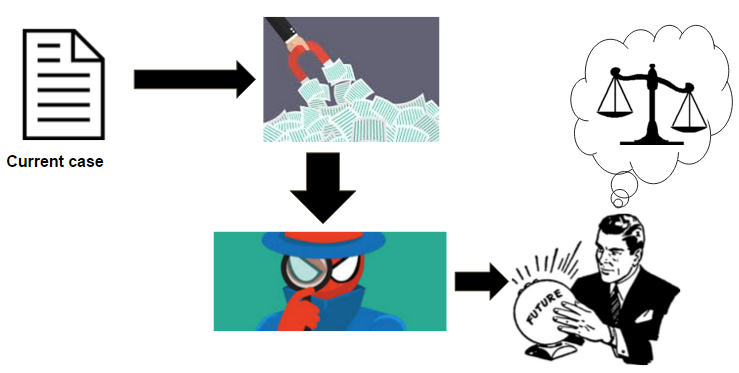
\includegraphics[width=\textwidth]{lawyerwork.PNG}
\end{frame}

\begin{frame}{Défis liés à la recherche et à l'analyse}
\begin{itemize}
\item Grande quantité des décisions: 2.5 Millions$^+$ par an
\item Documents non-structurés: pour l'automatisation
\item Complexité de l'organisation de la justice 
\item Compréhension difficile du langage juridique
\end{itemize}
\end{frame}

\begin{frame}{Thèse: un pipeline d'analyse de corpus jurisprudentiels}
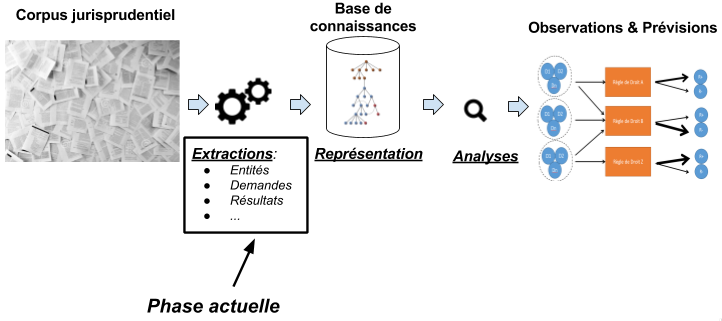
\includegraphics[width=\textwidth]{pipeline-cassandra2.png}
\end{frame}


\begin{frame}{Phase actuelle: Extraction d'information}
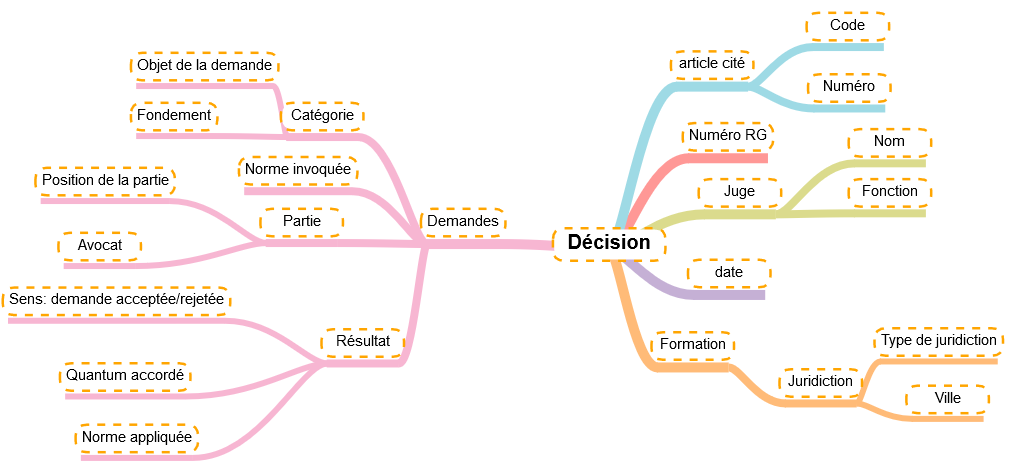
\includegraphics[width=0.9\paperwidth]{arbre-des-infos.PNG}
\end{frame}

\section{Détection de sections et d'entités}


\begin{frame}{Sectionner les décisions pour organiser l'extraction}
\scriptsize
\begin{columns}
\begin{column}{.45\linewidth}
\fbox{\begin{minipage}{\textwidth}ARRÊT N°

R.G: \textcolor{red}{11/03924}

\textcolor{red}{COUR D'APPEL} DE \textcolor{red}{NÎMES}

\textcolor{red}{CHAMBRE CIVILE}

\textcolor{red}{1ère Chambre A}

ARRÊT DU \textcolor{red}{20 MARS 2012}

APPELANTE:

\textcolor{red}{Madame Michéle A.} ...

assistée de la \textcolor{red}{SELARL VAJOU}, ...

INTIMES:

\textcolor{red}{Monsieur Martial B} ...

assisté de la \textcolor{red}{SCP MARION GUIZARD PATRICIA SERVAIS}, ...

COMPOSITION DE LA COUR LORS DU DÉLIBÉRÉ:

\textcolor{red}{M. Dominique BRUZY, Président}

\textcolor{red}{M. Serge BERTHET, Conseiller}

...
\end{minipage}}
\vspace{0.1cm}

{\normalsize \textbf{Entêtes}: méta-données}
\end{column}
\begin{column}{.55\linewidth}
\fbox{\begin{minipage}{\textwidth}FAITS, PROCEDURE, ...

Madame Michèle A. demande:

...

- de condamner Madame JONES-B. à lui payer la somme de \textcolor{red}{2.500 euros} au titre de l'\textcolor{red}{article 700 du Code de Procédure Civile}, 
\end{minipage}}
\vspace{0.1cm}

{\normalsize \textbf{Corps}: demandes, arguments et normes }

\vspace{0.4cm}

\fbox{\begin{minipage}{\textwidth}PAR CES MOTIFS, LA COUR:

...

Vu l'\textcolor{red}{article 809 du Code de Procédure Civile},

...

\textcolor{red}{Déboute Madame A. de sa demande de provision sur dommages-intérêts.}

...

Vu l'\textcolor{red}{article 700 du Code de Procédure Civile},

Condamne Madame JONES-B. à verser à Madame A. la somme de \textcolor{red}{2.500 euros}.
\end{minipage}}
\vspace{0.1cm}

{\normalsize \textbf{Dispositif}: résultats et normes}

\end{column}
\end{columns}
\end{frame}

%\begin{frame}{Entités et sections à détecter}
%
%\scriptsize
%\begin{table}[!htb]
%\centering
%%\scriptsize
%\begin{tabular}[c]{|l|c|p{0.6\textwidth}|}
%\hline
%\textbf{Entités} & \textbf{Labels} & \textbf{Exemples}\\\hline
%\multicolumn{3}{|c|}{\textbf{Section entête (E)}} \\
%\hline
%Numéro R.G. & \textbf{RG} & "10/02324", "60/JAF/09" \\ \hline
%Ville & \textbf{VL}& "NÎMES", "Agen", "Toulouse" \\ \hline
%Type de juridiction & \textbf{JR} & "COUR D'APPEL" \\ \hline
%Formation & \textbf{FM} & "1re chambre", "Chambre économique" \\ \hline
%Date & \textbf{DT} & "01 MARS 2012", "15/04/2014"\\ \hline
%Partie appelante & \textbf{AP} & "SARL K.", "Syndicat ...", "Mme X ..."\\ \hline
%Partie intimée & \textbf{IM} & - // - \\ \hline
%Partie intervenante & \textbf{IV} & - // - \\ \hline
%Avocat & \textbf{AV} & "Me Dominique A., avocat au barreau de Papeete"\\ \hline
%Juge & \textbf{JG} & "Monsieur André R.", "Mme BOUSQUEL" \\ \hline
%fonction du juge & \textbf{FT} & "Conseiller", "Président"\\ \hline
%\multicolumn{3}{|c|}{\textbf{Corps (T) et dispositif (D)}} \\ \hline
%
%Norme & \textbf{NO} & "l' article 700 NCPC", "articles 901 et 903"  \\ \hline
%\hline
%Élément à éviter & \textbf{O} & \textit{tout élément ne faisant partie d'aucune entité ciblée} \\ \hline
%\end{tabular} 
%
%\caption{Entités et leurs labels par section.}\label{relevantinfo}
%\end{table}
%\end{frame}

\begin{frame}{Approches probabilistes d'étiquetage de séquence}
Modèles probabilistes à états et observations

\scriptsize
\begin{table}[]%width=\linewidth
	%\begin{tabular}[]{p{0.40\linewidth}|p{0.55\linewidth}}
	\begin{tabular}[]{c|c}
		\toprule
{\textbf{HMM}} & {\textbf{CRF}} \\
%		\midrule
%		\textbf{Generative} models 	& \multicolumn{2}{c}{"\textbf{Discriminative}" or "\textbf{Conditional}" models } \\[0.25em]
%\midrule		
%"\textbf{generate}" input	& {"\textbf{condition}" on input }\\%[0.25em]
\midrule
{un seul descripteur  par observation}	& {plusieurs descripteurs complexes par observation}\\%[0.25em]
\midrule	
		\begin{tikzpicture}[->,>=stealth',shorten >=1pt,auto,node distance=1.3cm,
                    semithick]
  \node[state] (S1)                    {$s_{t-1}$};
  \node[state]         (S2) [right of=S1] 	  {$s_{t}$};
  \node[state]         (O) [below of=S2] {$o_{t}$};
  \path (S1) edge              node {} (S2)
        (S2) edge              node {} (O);
\end{tikzpicture}
				& 

\begin{tikzpicture}[auto,>=stealth',shorten >=1pt,auto,node distance=1.3cm,
                    semithick]
  \node[state] (S1)                    {$s_{t-1}$};
  \node[state]         (S2) [right of=S1] 	  {$s_{t}$};
  \node[state]         (O) [below of=S2] {$o_{t}$};
  \path (S1) edge              node {} (S2)
        (S2) edge              node {} (O);
\end{tikzpicture}					
					\\%[0.25em]
\midrule
$P_\lambda(S,O) = \prod\limits_{t=1}^{T} P(s_t \vert s_{t-1}) * P(o_t \vert s_{t})$  & $P_\lambda(S|O) = \frac{1}{Z(O)}exp\left( \sum\limits_{t=1}^{T}\sum\limits_{k} \lambda_k f_k(s_{t-1},s_t, o_t) \right) $ \\
% & & & \\
\tiny \cite{Seymore1999hmm} & \tiny \cite{peng2006crf} \\ 
		\bottomrule
	\end{tabular}
\end{table}

\normalsize

Objectif: Trouver la séquence la plus probable d'étiquetage pour l'ensemble du texte

\textbf{Entrainement fait sur des séquences préalablement étiquetées}
\end{frame}

\begin{frame}{Sélection des caractéristiques}
\tiny
\begin{tabular}{l|c|ccc}
\toprule
Detection Task & Tagger & {Token-level F1$^a$} & {Entity-level F1$^a$}& Features subset \\ 
\midrule
\multirow{7}{*}{Sections} 		& \multirow{4}{*}{CRF} & 99.31 & 90.48 & BDS$^{b1}$  \\
  				&  & \textbf{99.55} & 85.76 & \textbf{SFFS}$^{b2}$ \\
                &  & 99.46 & 90.03 & ALL \\
                &  & 91.75 & 60.26 & token \\  \cline{2-5}
                 & \multirow{3}{*}{HMM} & \textbf{90.99} & 3.89 & \textbf{absLength} \\ 
 & & 86.97 & 3.65 & relLength \\   
  &  & 37.59 & 18.81 & token \\ \hline
\multirow{7}{*}{Header entities}	& \multirow{4}{*}{CRF} & 92.69 & 90.47 & BDS$^{c1}$  \\
				&  & \textbf{93.00} & 90.76 & \textbf{SFFS}$^{c2}$  \\ 
                &  & 92.74 & 90.81 & ALL \\
                &  & 82.73 & 72.17 & token \\ \cline{2-5}
                  &  \multirow{3}{*}{HMM}  & \textbf{78.61} & \textbf{56.93} &  \textbf{token} \\ 
  &    & 68.04 & 32.96 &  lemma\_W0 \\ 
  &    & 38.54 & 7.95 &  POS \\ \hline
\multirow{6}{*}{Norms} 			& \multirow{4}{*}{CRF} & \textbf{96.31} & 90.80 & \textbf{BDS}$^{d1}$ \\ 
				&  & 95.57 & 89.29 & SFFS$^{d2}$ \\ 
                &  & 95.87 & 90.76 & ALL \\
                &  & 94.26 & 85.72 & token \\ \cline{2-5}
                 &  \multirow{2}{*}{HMM} & \textbf{91.66} & \textbf{74.9} &  \textbf{token} \\ 
  &   & 91.54 & 69.35 &  lemma\_W0 \\ 
%  \noalign{\smallskip}\svhline\noalign{\smallskip}
%  & & token-level & entity-level & \\ \hline
\bottomrule
\end{tabular}
\end{frame}

\begin{frame}{Sélection de la représentation de segment}
\tiny
\begin{tabular}{p{0.17\textwidth}|c|cccp{0.18\textwidth}}
\toprule
Detection Task & Tagger\hspace{0.1cm} & {Token-level F1$^a$}\hspace{0.1cm} & {Entity-level F1$^a$}\hspace{0.1cm} & training time$^b$\hspace{0.1cm} & Representation \\ 
\midrule
\multirow{8}{*}{Sections}  & \multirow{4}{*}{CRF} & 91.75 & 60.26 &  4.685  & IO \\
&  & 88.95 & 42.63  & 11.877 & IEO2 \\
&  & 87.09 & 41.45 & 12.256 & BIO2 \\
 &  & 86.00 & 48.97  & 35.981 & BIEO \\ \cline{2-6}
& \multirow{4}{*}{HMM} & 32.64 & 20.41 & 6.564 & IO \\
&  & 32.92 & 16.87  &   7.827  & IEO2 \\
 &  & 32.39 & 29.05 & 8.391 & BIO2 \\
  &  & 33.06 & 29.80 & 8.7 & BIEO \\ \hline %
\multirow{8}{*}{Header entities}  & \multirow{4}{*}{CRF} & 82.73 & 72.17  & 70.525 & IO \\
 &  & 83.51 & 72.82  & 228.751 & IEO2 \\
 &  & 82.51 & 73.49 & 230.865 & BIO2 \\
 &  & 83.44 & 75.53 &  475.249 & BIEO \\ \cline{2-6}
  & \multirow{4}{*}{HMM} & 73.00 & 44.64 & 6.345 & IO \\
  &  & 73.40 & 50.11& 8.298 & IEO2 \\ 
  &  & 73.49 & 55.14 & 7.908 & BIO2 \\
 &  & 74.12 & 60.46 & 9.973 & BIEO \\ \hline
\multirow{8}{*}{Norms}  & \multirow{4}{*}{CRF} & 94.26 & 85.72 & 28 & IO \\%
&  & 94.27 & 87.17 & 32.136 & IEO2 \\
 &  & 94.24 & 84.37 & 50.769 & BIO2 \\
  &  & 93.47 & 86.72 & 50.566 & BIEO \\ \cline{2-6}
  & \multirow{4}{*}{HMM} & 89.30 & 74.37 &  41.389 & IO \\%  
   &  & 88.71 & 79.61 & 44.086 & IEO2 \\
  &  & 88.53 & 75.24 & 46.634 & BIO2 \\
  &  & 87.74 & 79.99 & 45.52& BIEO \\
\bottomrule
\end{tabular}
\end{frame}

\begin{frame}{Nombre nécessaire de données d'entrainement}
\begin{figure}[!h]
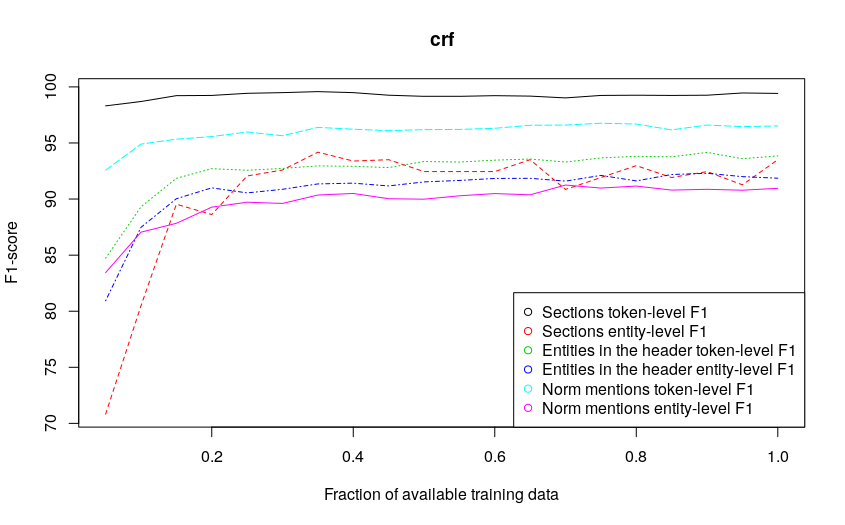
\includegraphics[width=0.9\textwidth]{lc-crf.png}
\caption{Résultats en fonction du nombre de données d'entrainement (fractions d'environ 380 décisions)}\label{p4_crf-learning-curves}
\end{figure}
\end{frame}

\section{Extraction d'informations sur les demandes}

\begin{frame}{Extraction des informations sur les demandes}
\begin{block}{Informations pertinentes à extraire}
\begin{itemize}
\item \textbf{Position de la partie}: Intimé
\item \textbf{Catégorie de demande}: Dommages-intérêts pour procédure abusive
\begin{itemize}
\item \textbf{Objet}: Dommages-intérêts
\item \textbf{Fondement}: Articles 1382 code civil et 32-1 code de procédure civile
\end{itemize}
\item \textbf{Quantum demandé}: 20 000 euros
\item \textbf{Résultat} : Rejet
\item \textbf{Quantum accordé} : 0 euros
\end{itemize}
\end{block}
\end{frame}

\begin{frame}{Difficultés (1)}

Expressions explicite / implicite

\begin{alertblock}{Exemple: Expression de demande}
La société A. conclut à la confirmation du jugement entrepris sauf à
former appel incident sur la disposition du jugement l'ayant déboutée de sa
demande de \textbf{dommages intérêts pour abus de procédure} et elle demande à la cour de
condamner l'appelante à lui payer la somme de \textbf{20 000 euros} à titre de dommages
intérêts ...

%- \textbf{la} condamner à payer une somme de \textbf{283 589 euros} à titre de {\bf dommages et intérêts pour concurrence déloyale},

...
\end{alertblock}

\begin{alertblock}{Expression de resultat}
La cour, ... 

\textbf{Confirme la décision entreprise en toutes ses dispositions},
\end{alertblock}
\end{frame}

\begin{frame}{Difficultés (2)}

\begin{alertblock}{}
\begin{itemize}
\item Plusieurs catégories similaires ou différentes dans une décision
\item Toutes les catégories ne sont pas connues d'avance
\end{itemize}
\end{alertblock}
\end{frame}


\begin{frame}{Approche supervisée d'extraction des demandes}
\begin{alertblock}{Simplification du probleme}
\begin{itemize}
\item On suppose qu'une décision ne comprend qu'au plus une demande d'une catégorie donnée
\item Méthode générique qui s'adapte aux spécificités de la catégorie traitée
\item Création incrémentale des catégories
\end{itemize}
\end{alertblock}

%\begin{block}{Définition d'une classe de décision}
%Soit $C$ une catégorie de demande et $D$ une décision,
%
%s'il existe dans $D$ une demande $d$ de catégorie $C$, alors $C$ est une classe de $D$
%\end{block}
\end{frame}

%\begin{frame}{Détection d'une catégorie par classification}
%\begin{figure}
%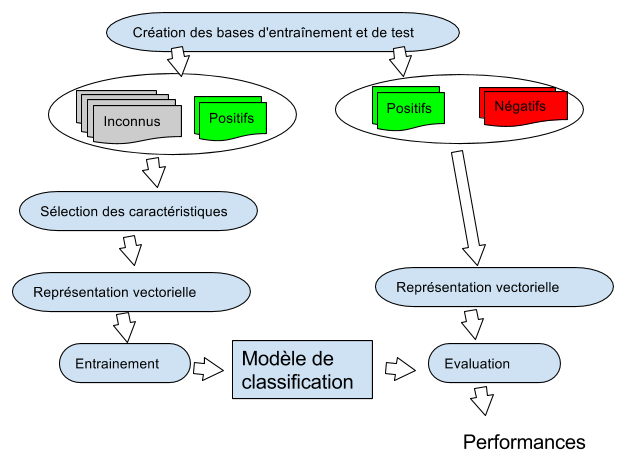
\includegraphics[scale=0.6]{archi-classif.png}
%\caption{Approche d'expérimentation de la classification}
%\end{figure}
%\end{frame}

\begin{frame}{Détection d'une catégorie par classification}
(1) Sélection de termes caractéristique
\begin{exampleblock}{Dommages-interets pour abus de procedure}
\small
\begin{tabular}{l|c}
\textbf{Terme (n-gram)} & \textbf{Poids global (NGL)}  \\ \hline
\midrule
procédure abusive & 15.710 \\ \hline
pour procédure abusive & 15.007 \\ \hline
pour procédure & 14.890 \\ \hline
abusive & 13.721 \\ \hline
intérêts pour procédure & 10.306 \\ \hline
abus & 10.288 \\ \hline
intérêts pour procédure abusive & 9.984 \\ \hline
32-1 & 9.534\\ \hline
%et intérêts pour procédure & 9.341 \\ \hline
%dommages et intérêts pour procédure & 9.341 \\ \hline
... & ...
\end{tabular}
\end{exampleblock}
$ngl(w,c) = \frac{\sqrt{N} ((N_{w,c} N_{\overline{w},\overline{c}}) - (N_{w,\overline{c}} N_{\overline{w},c}))}{\sqrt{N_w N_{\overline{w}} N_c N_{\overline{c}}}}$ \cite{ng1997ngl}
\end{frame}

%\begin{frame}{Catégorisation semi-supervisée des décisions}
%\begin{figure}
%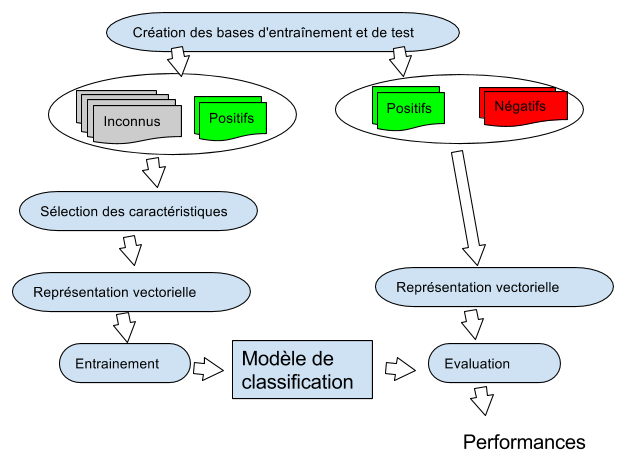
\includegraphics[scale=0.6]{archi-classif.png}
%\caption{Approche d'expérimentation de la classification}
%\end{figure}
%\end{frame}

\begin{frame}{Détection d'une catégorie par classification}
(2) Représentation vectorielle \& Classification des décisions
\begin{figure}
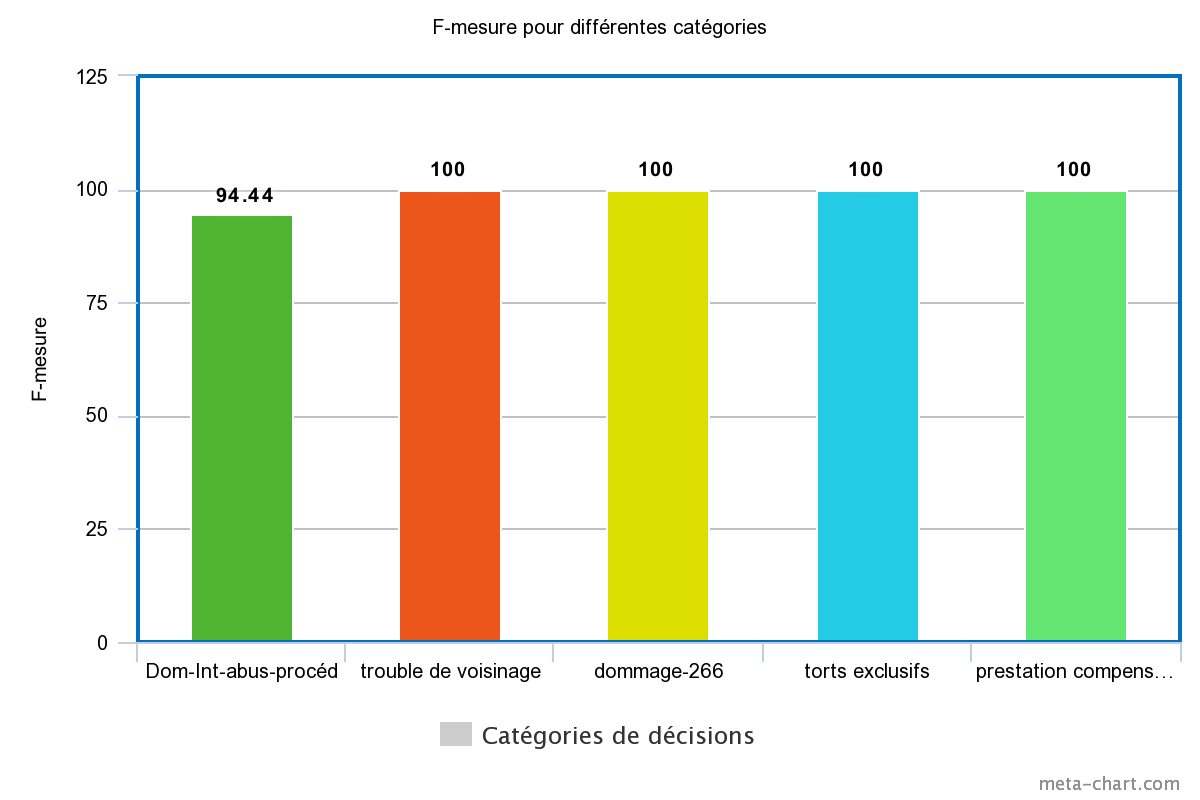
\includegraphics[width=0.8\textwidth]{f-mesure-classif.png}
\caption{Résultats des meilleures configurations (taille des vecteurs, poids global, poids local, modèle de classifieur)}
\end{figure}
\end{frame}

\begin{frame}{Interprétation des résultats pour une catégorie}
Tentative par classification des décisions
\begin{figure}
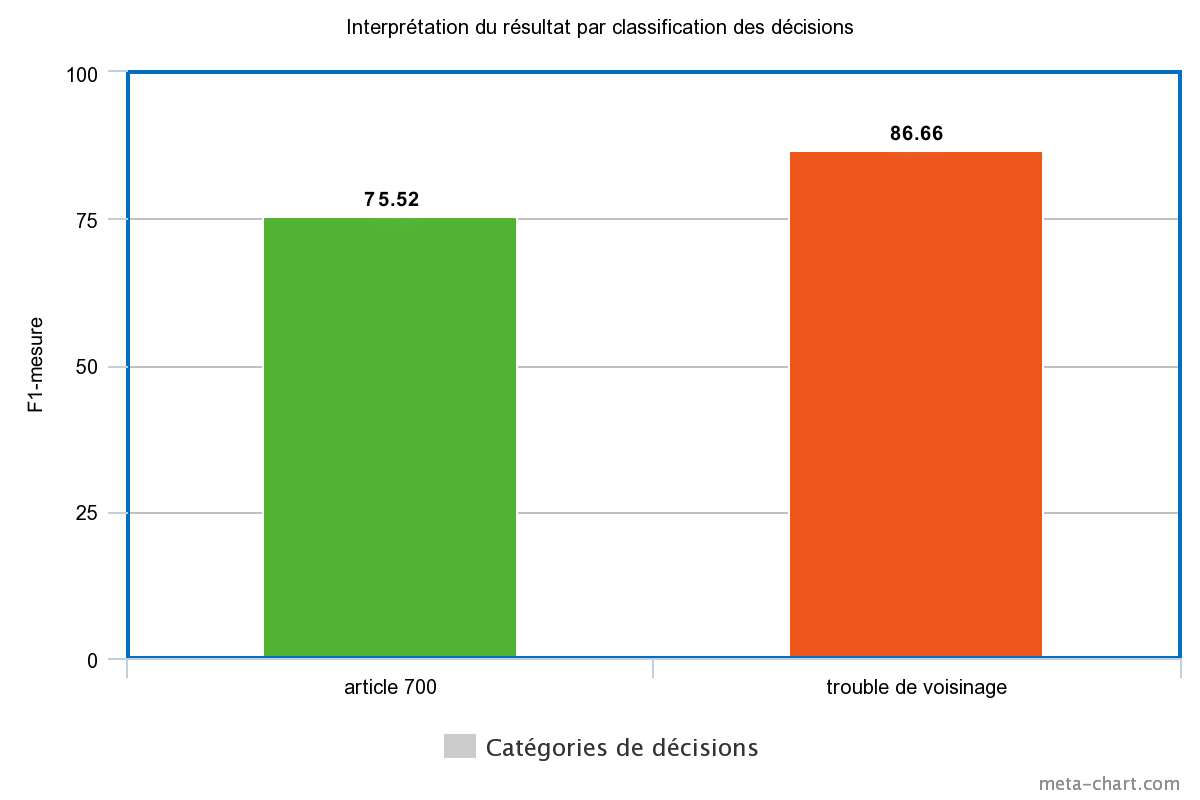
\includegraphics[width=0.8\textwidth]{classifResultat.png}
\caption{Résultats des meilleures configurations (taille des vecteurs, poids global, poids local, modèle de classifieur)}
\end{figure}
\end{frame}

\section{Directions futures}

\begin{frame}{(1) Extraction des demandes et résultats}

\end{frame}

\begin{frame}{(2) Analyse de la sémantique des demandes et résultats}

(2.a) Catégorisation des demandes:
\begin{itemize}
\item supervisée: classifier les demandes dans des catégories prédéfinies par des experts juristes
\item non-supervisée: suggérer des regroupements assez similaires aux catégories prédéfinies
\end{itemize}


(2.b) Interprétation des résultats: 

\textit{ACCEPTE / REJETTE / NE SE PRONONCE PAS}


\end{frame}

\begin{frame}{(3) Standardisation et représentation des connaissances}
\begin{figure}
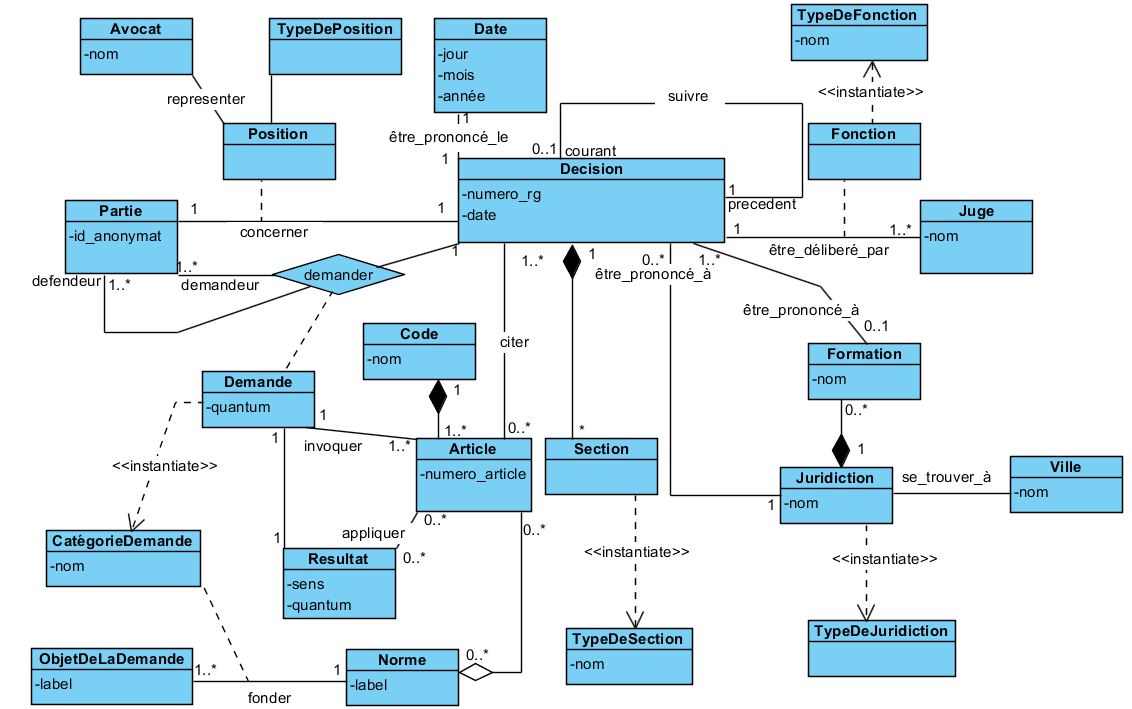
\includegraphics[width=0.7\paperwidth]{class-diagram.png}
%\caption{Modèle des données}
\end{figure}

Désambiguïsation et résolution d'entités?

BD Relationnelle ou Linked Data ou autre?
\end{frame}

\begin{frame}{(4) Analyser la prise de décision des juges?}


Quels facteurs explicatifs?

Quelles relations entre les quanta demandés et les quanta accordés?

Extraire et analyser :

\begin{itemize}
\item  les arguments > \textit{corrélation avec le sens des résultats}

\item les circonstances factuelles > \textit{clustering des décisions et topic modeling}

\item les quanta 

\end{itemize}

\end{frame}


%%-=-=-=-=-=-=-=-=-=-=-=-=-=-=-=-=-=-=-=-=-=-=-=-=
%%
%%	Questions
%%
%%-=-=-=-=-=-=-=-=-=-=-=-=-=-=-=-=-=-=-=-=-=-=-=-=
\section{Questions?}
%-=-=-=-=-=-=-=-=-=-=-=-=-=-=-=-=-=-=-=-=-=-=-=-=
%	References:
%-=-=-=-=-=-=-=-=-=-=-=-=-=-=-=-=-=-=-=-=-=-=-=-=
\begin{frame}[t,allowframebreaks]{References}
\tiny
\bibliographystyle{apalike}
\bibliography{references}	
\end{frame}

\end{document}
